\documentclass[tikz,border=2pt]{standalone}
\usepackage{pgfplots}
\pgfplotsset{compat=1.18}

\begin{document}
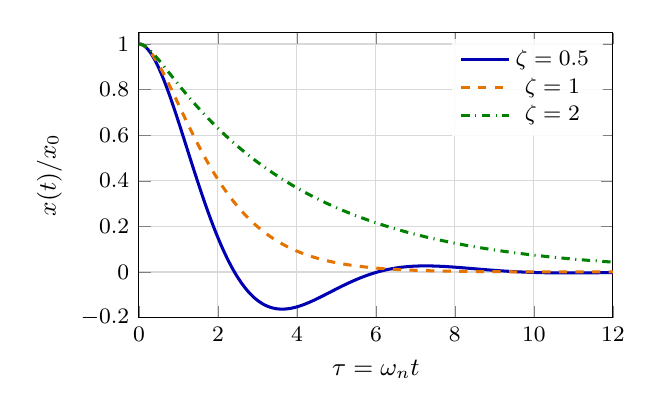
\begin{tikzpicture}
\begin{axis}[
    width=7.6cm,
    height=5.2cm,
    xmin=0,
    xmax=12,
    ymin=-0.2,
    ymax=1.05,
    xlabel={$\tau=\omega_n t$},
    ylabel={$x(t)/x_0$},
    xtick={0,2,4,6,8,10,12},
    ytick={-0.2,0,0.2,0.4,0.6,0.8,1.0},
    grid=both,
    major grid style={draw=gray!30},
    tick label style={font=\footnotesize},
    label style={font=\small},
    legend style={
        at={(0.98,0.98)},
        anchor=north east,
        draw=none,
        fill=white,
        fill opacity=0.88,
        text opacity=1,
        font=\footnotesize,
        row sep=-1pt
    }
]
\addplot[
    blue!70!black,
    line width=1.1pt,
    domain=0:12,
    samples=500
] {exp(-0.5*x)*(cos(deg(sqrt(0.75)*x))+(0.5/sqrt(0.75))*sin(deg(sqrt(0.75)*x)))};
\addlegendentry{$\zeta=0.5$}

\addplot[
    orange!90!black,
    dashed,
    line width=1.1pt,
    domain=0:12,
    samples=500
] {(1+x)*exp(-x)};
\addlegendentry{$\zeta=1$}

\addplot[
    green!50!black,
    dashdotted,
    line width=1.1pt,
    domain=0:12,
    samples=500
] {0.5*(1-2/sqrt(3))*exp((-2-sqrt(3))*x)+0.5*(1+2/sqrt(3))*exp((-2+sqrt(3))*x)};
\addlegendentry{$\zeta=2$}
\end{axis}
\end{tikzpicture}
\end{document}
